\section*{Dati e risultati}

\subsection*{Tempo di propagazione di un segnale}

In questa sezione della relazione vogliamo studiare il tempo di propagazione di un segnale all'interno di una porta logica. Nel nostro caso useremo porte NAND.

Prima di procedere, è doveroso chiarire come mai la risposta della porta ad una variazione del segnale e alla sua propagazione non sia immediata.
Per rispondere a questa domanda ome prima cosa è doveroso ricordare che tutte le porte logiche che tilizziamo e andeamo ad utilizzare sono basate sulla Logica Transistor-Transistor o in forma abbreviata logica TTL. Pertanto le porte utilizzate logiche sono implementate tramite reti di transistor e resistenze opportunamente interconnessi. Quindi l'intera rete presenta delle giunzioni che come sappiamo possono assumere il ruolo di fastidiose capacità parassite. E naturalmente una caparità per quanto piccola possa essere produce sempre un ritardo nella propagazione di un segnale.

Detto questo possiamo andare a realizzare il circuito che ci permette di apprezzare questo ritardo nella trasmissione del segnale. Il circuito è raffigurato in Figura \ref{fig:ritardo}. Con questo circuito vogliamo amplificare questo effetto di ritardo solo su uno dei due ingressi della quarta porta NAND. In questo modo possiamo capire infatti se sussiste un ritardo e, se sì, quanto vale indicativamente. Come possiamo osservare le porte NAND così connesse non sono altro che una serie di NOT messi in cascata.

Inoltre ricordiamo quale sia la tabella di verità di una porte NAND:

\begin{center}
	\begin{tabular}{lll}
	\toprule
		A & B & O\\
	\midrule
		0 & 0 & 1 \\
		0 & 1 & 1 \\
		1 & 0 & 1 \\
		1 & 1 & 0 \\
	\bottomrule
	\end{tabular}
\end{center}
%
Quindi in base alla geometria del circuito che abbiamo realizzato, dato un segnale A di ingresso, l'uscita del circuito dovrebbe assumere lo stesso valore dell'ingresso. Infatti se anlizziamo la tabella di verità di questo circuito otteniamo quanto illustrato nella Tabela \ref{tab:ritardo}.

\begin{wrapfloat}{table}{I}{300pt}
\centering
	\begin{tabular}{l | llll | l}
	\toprule
		In & A & B & C & D & Out\\
	\midrule
		1 & 0 & 1 & 0 & 1 & 1 \\
		0 & 1 & 0 & 1 & 0 & 1 \\
	\bottomrule
	\end{tabular}
	\caption{Tabella di verità del circuito in Figura \ref{fig:ritardo}}
	\label{tab:ritardo}
\end{wrapfloat}

Nella Tabella \ref{tab:ritardo} abbiamo indicato con In il valore del segnale in ingresso al circuito, con Out il valore del segnale in uscita dallo stesso e le altre lettere sono riferite alle uscite delle varie porte NAND riportate in Figura \ref{fig:ritardo}.

Andiamo ora a verificare sperimentalmente che la tabela di verità sia corretta. A tal fine abbiamo Connesso l'ingresso del circuito al generatore di funzioni. Abbiamo dato come segnale in input un'onda quadra di frequenza $f\,=\,\SI{100}{\kilo\hertz}$ di ampiezza \SI{2.5}{\volt} con una tensione di offset di \SI{1.25}{\volt}. Dopo di chè abbiamo connesso l'uscita del circuito all'oscilloscopio e siamo andati a osservare il comportamento del segnale in uscita.

Quello che abbiamo ottenuto è riportato in Figura \ref{fig:ritardo1_plot}:

Come è possibile osservare dal grafico in Figura \ref{fig:ritardo1} l'uscita del nostro circuito non è quella prevista, o meglio, lo sarebbe a meno di un piccolo intervallo temporale in cui l'uscita del circuito assume valore di verità nullo. Questo è dovuto appunto alla presenza delle capacità parassite interne alle porte logiche che rallentano la trasmissione del segnale. Infatti se si parte con un segnale in ingresso ad 0 logico, sugli ingressi della quarta porta NAND (C e D) giungeranno i valori di verità 1 e 0 rispettivamente. Pertanto l'uscita del circuito deve essere ad 1 logico, trattandosi di una porta NAND. Nel momento in cui il segnale in ingresso assume valore di verità 1 abbiamo un ritardo nella trasmissione della variazione in uno dei due ingressi della quarta porta NAND. Per questo motivo, per un breve intervallo temporale, stimato circa XXX, abbiamo la seguente situazione: In = 1, C = 1 (a causa del ritardo di trasmissione del segnale ha ancora il valore di verità relativo al segnale in ingresso precedente), D = 1 e quindi Out = 0. Quindi questa è la spiegazione per la breve variazione di tensione in uscita dal circuito. Infine facciamo notare che questo fenomeno non occorre quando l'input passa da 1 a 0 in quanto si avrebbe che C = 0 e D = 0 quindi Out = 1.

\subsection*{Porta NOT TTL Open Collector}

In questa sezione vogliamo verificare il corretto funzionamento di una porta NOT con tecnologia TTL Open Collector, modello SN74LS05N. Una porta NOT TTL Open Collector si può schemattizzare come un transistor. Il segnale in ingresso alla base è l'input della porta logica, mentre il collettore è l'output della porta logica.
Detto questo passiamo alla realizzazione del circuito: Figura \ref{fig:not}.
Dal momento che vogliamo pilotare un LED dobbiamo anche prestare attenzione alle sue caratteistihe, in modo da non farci passare una corrente eccessiva e rischiare pertanto di bruciarlo. A tal fine abbiamo dimensionato il circuito sapendo che: c'è una caduta di tensione di \SI{1}{\volt} sul LED in conduzione, l'intensità di corrente indicata che dovrebbe scorrere sul LED è di \SI{5}{\milli\ampere}, una caduta di \SI{0.4}{\volt} tra collettore ed emettitore del transistor e l'alimentazione del collettore a \SI{9}{\volt}. Quindi trammite una serie di calcoli elementari abbiamo ottenuto che il valore di resistenza $R$ teorico deve essere di circa \SI{1.52}{\kilo\ohm}. Tuttavia abbiamo deciso di realizzare la nostra resistenza con una resistenza da \SI{1}{\kilo\ohm} in serie con un trimmer. In questo modo, grazie al multimetro, abbiamo regolato il trimmer in modo da avere esattamente \SI{5}{\milli\ampere} di corrente passanti sul LED. Il valore di resistenza sperimentale trovaro vale: $R\,=\,\SI{1.34}{\kilo\ohm}$.

Quindi a questo punto siamo andati a verificare il corretto funzionamento della nostra porta NOT TTL Open collector. Abbiamo ottenuto che quando in input il segnale è ad 1 logico, ovvero \SI{5}{\volt} il LED è acceso quindi l'uscita è all'1 logico, mentre quando l'input si trova allo 0 logico il LED è anch'esso spento, 0 ogico.
Questo comportamento è corretto. Infatti quando l'input è ad 1 logico, il transistor è in conduzione e l'uscita si trova a circa \SI{0.4}{\volt} che è ancora 0 logico, pertanto c'è una differenza di potenziale ei cali del LED e questo si accende. Al contrario, quando l'input è allo 0 logico, il ransistor è interdetto, non scorre corrente, quindi il collettore sarà ad una tensione di circa \SI{9}{\volt} quindi ad 1 logico. Pertanto non passando corrente il LED è spento.

\subsection*{Porta buffer TTL 3State}

In questa sezione vogliamo verificare il corretto funzionamento di una porta buffer TTL 3-state modello 74LS125A. Per farlo realizziamo un circuito per trasmissione half-duplex tramite porte 3-state al fine di condividere lo stesso canale trasmissivo. Circuito riportato in Figura \ref{fig:buffer}. Quindi fatta la tabela di verità di tale circuito ne verificheremo la correttezza.

Ricordiamo che in elettronica digitale, una porta logica si dice three state, tri-state o 3-state quando la sua uscita può trovarsi in un terzo stato di alta impedenza (Z) oltre ai due livelli logici della logica binaria.
Uno dei principali dispositivi a tre stati è il buffer a tre stati (o buffer tri-state). La sua tabella di verità è la seguente:

\begin{center}
	\begin{tabular}{lll}
	\toprule
		B & In & Out\\
	\midrule
		0 & 0 & Z \\
		0 & 1 & Z \\
		1 & 0 & 0 \\
		1 & 1 & 1 \\
	\bottomrule
	\end{tabular}
\end{center}
%
dove con In abbiamo indicato lo stadio di ingresso, con B il segnale di pilotaggio e Out indica l'output della porta.
Quindi un buffer tri-state può essere pensato come interruttore. Se B è acceso, l'interruttore è chiuso e il segnale in ingresso viene trasmesso; se B è spento, l'interruttore è aperto e l'uscita si trova ad alta impedenza.

La tabella di verità del circuito in Figura \ref{fig:buffer} è la seguente:

\begin{center}
	\begin{tabular}{lllll}
	\toprule
		In & B & A & C & O\\
	\midrule
		0 & 0 & 0 & 0 & 0 \\
		1 & 0 & 1 & 0 & 1 \\
		0 & 1 & Z & 0 & 0 \\
		1 & 1 & Z & 0 & 0 \\
	\bottomrule
	\end{tabular}
\end{center}
%
Tale tabella è stata conferata anche dall'analisi sperimentale del circuito. Circuito che riceve ininput un onda quadra, con frequenza a scelta di ampezza \SI{2.5}{\volt} e offset di \SI{1.25}{\volt}. 

\subsection*{Multiplexing}

In questa ultima sezione il nostro obbiettivo è quello di realizzare un Multiplexing. Che cosa è? In parole povere è un dispositivo che permette a segnali in ingresso (detti tributari) tramite canali separati, quindi distinti tra di loro, di essere trasmessi mediante un solo segnale in uscita (detto multiplato). Quindi la trasmissione di numerosi segnali viene effettuata da un unico collegamento fisico. In questo modo non occorre associare ad ogni input un output differente, ma si riesce a convogliare tutto il segnale in unica uscita.

Tale circuito si può schematizzare in due blocchi principali: i primo blocco è quello di selezione, mentre il secondo blocco è quello di ``gating''. 
Questi due blocchi sono raffigurati in Figura BHO.

\paragraph*{Blocco di selezione:}
la sua configurazione circuitale è riportata in Fugura XXX. Questo blocco sfrutta le proprieta delle porte logiche NOT e NAND. Grazie a queste porte io con due segnali in in ingresso posso ottenere quattro uscite che non sono mai contemporaneamente spente, o a 0 logico. Quindi, se io indico con $S_0$ e $S_1$ le due linee di selezione che abbiamo deciso di utilizzare (input), posso ottenere la seguente tabella di verità, dove con $Q_i$ abbiamo indicato le uscite del selettore.

\begin{center}
	\begin{tabular}{ll|llll}
	\toprule
		$S_0$ & $S_1$ & $Q_0$ & $Q_1$ & $Q_2$ & $Q_3$ \\
	\midrule
		0 & 0 & 0 & 1 & 1 & 1 \\
		0 & 1 & 1 & 0 & 1 & 1 \\
		1 & 0 & 1 & 1 & 0 & 1 \\
		1 & 1 & 1 & 1 & 1 & 0 \\
	\bottomrule
	\end{tabular}
\end{center}

Indichiamo con $D_i$ i segnali che devono essere trasmessi. Questo primo blocco diventa pertanto una sorta di interruttore che mi permette di decidere quale segnale in ingresso ($D_i$) trasmettere lungo la linea dati comune. Pertanto a seconda dei valori che io imposto di $S_0$ ed $S_1$ posso decidere se trasmettere il segnale $D_0$ o $D_2$ ad esempio, ma mai due di questi contemporaneamente. Questo processo avviene grazie al secondo blocco detto di ``gating''.

\paragraph*{Blocco di ``gating'':}
questo blocco, illustrato in Figura XXX, è la parte di circuito che effettivamente permette o meno il passaggio dei dati, Indicati con $D_i$. Come già detto in precedenza sfruttando la porta porta buffer TTL 3State possiamo ottenere degli interruttori. Quindi se ad ogni $D_i$ accoppiamo il $Q_i$ corrispondente, per evitare confusione, otteniamo un interruttore che a seconda del valore assunto da $Q_i$ permette o meno la trasmissione del segnale. $Q_i\,=\,0$ il segnale è trasmesso se $Q_i\,=\,1$ il segnale non è trasmesso. Quindi, farendo riferimento alla tabella di verità del selettore, possiamo osservare come sia possibile permettere il passaggio di un solo segnale alla volta in un unica linea dati in uscita dal ``gating''.

Quanto appena descritto è il funzionamento del nostro multiplexing.















%\begin{wrapfloat}{figure}{I}{0pt}
%\includegraphics[width=0.5\textwidth]{Relativo}
%\caption{Esempio di figura ‘‘avvolta’’ da un testo.}
%\end{wrapfloat}

%\begin{center}
%	\begin{tabular}{lll}
%	\toprule
%		A & B & C \\
%	\midrule
%		& & \\
%		& & \\
%		& & \\
%		& & \\
%	\bottomrule
%	\end{tabular}
%\end{center}

%\begin{figure}[t!]
%    \centering
%    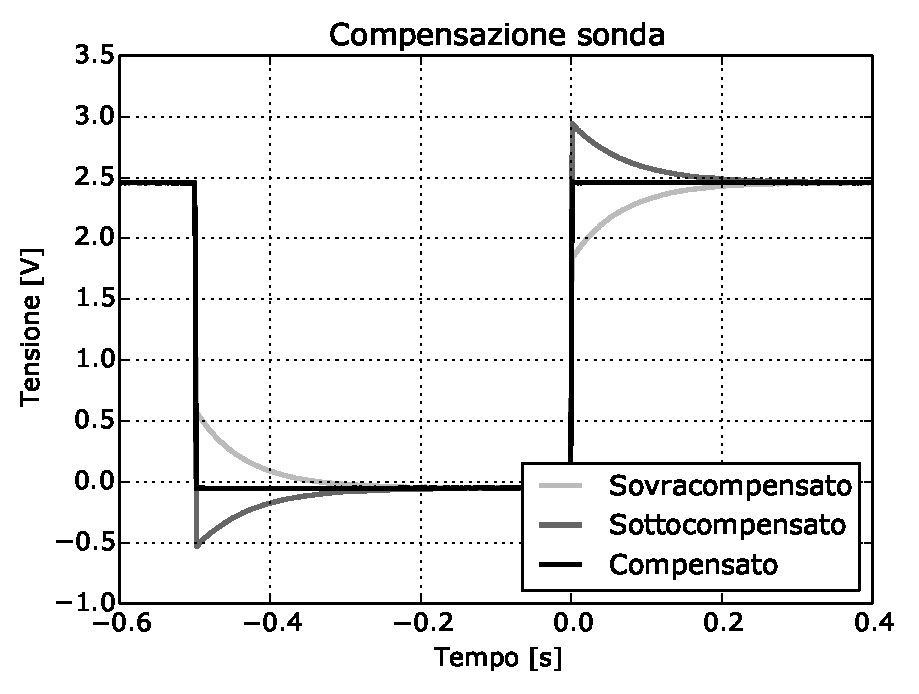
\includegraphics[width=\columnwidth]{figure/comp.pdf}
%    \caption{Input dell'oscilloscopio con una sonda compensabile. Cambiando capacità
%        si può ottenere una sottocompensazione, una sovracompensazione oppure compensare perfettamente
%        le capacità, ottenendo un'onda quadra.}
%    \label{fig:compensazione}
%\end{figure}

%\begin{wrapfloat}{figure}{O}{0pt}
%        \def\svgwidth{0.4\textwidth}
%        \subimport{figure/}{raddrizzatore.pdf_tex}
%        \caption{Raddrizzatore di precisione a semionda. Alimentato, inizialmente con una $V\ped{in}\,=\,\SI{1.02}{\volt}$ di frequenza $\nu\,=\,\SI{50}{\hertz}$.}
%        \label{fig:radd}
%\end{wrapfloat}

%\begin{SCfigure}[][p]
%        \centering
%        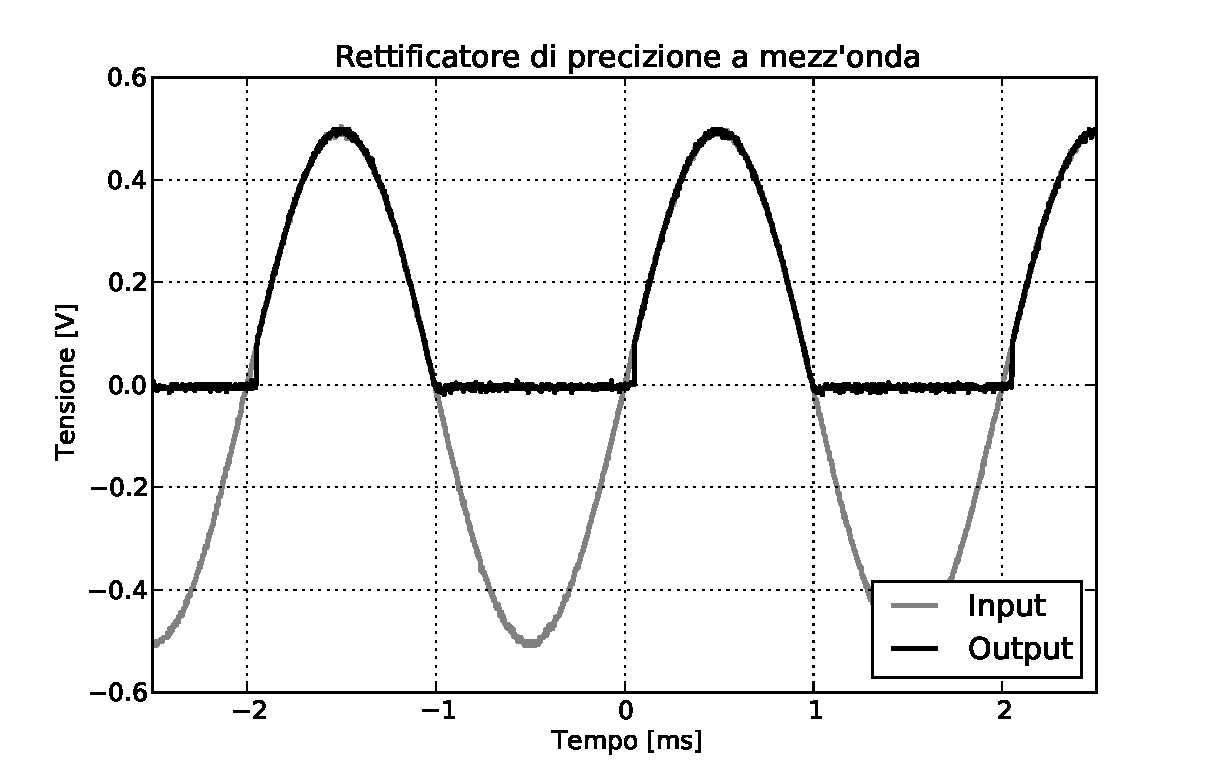
\includegraphics[width=0.7\textwidth]{figure/rett.pdf}
%        \caption{Questo grafico illustra l'andamento di $V\ped{out}$, linea nera, in funzione di $V\ped{in}$, linea grigia. Si nota chiaramente, come da previsioni, che la parte negativa del segnale in ingresso impediscse al diodo di condurre, pertanto la tensione di output risulta nulla. Inoltre, come si può osservare, il fronte di salita di $V\ped{out}$ presenta un leggero ritardo rispetto al segnale in ingresso $V\ped{in}$. Questo ritardo è stato stimato essere approssimativamente di circa $(152\pm10)\SI{}{\micro\second}$.}
%        \label{fig:radd_plot1}
%\end{SCfigure}
